\documentclass[11pt]{article}
\usepackage[a4paper,margin=2.2cm]{geometry}
\usepackage{booktabs}
\usepackage{longtable}
\usepackage{pdflscape}
\usepackage{amsmath}
\usepackage{graphicx}
\usepackage{hyperref}
\usepackage{tikz}
\usetikzlibrary{arrows.meta,positioning,shapes.geometric,calc}

\title{MORPHEUS model construction for semiexperimental structures: coordinates, constraints, classes, and predicates}
\author{MATRIX/MORPHEUS working draft}
\date{\today}

\begin{document}
\maketitle

\begin{abstract}
Semiexperimental equilibrium structures are often limited less by the least-squares
algorithm than by the definition of the refinement model.  MORPHEUS treats model
construction as an explicit, auditable step.  The user may refine in symmetry-adapted
generalized internal coordinates (GICs) or in symmetry-adapted Cartesian coordinates,
while chemical knowledge is always expressed at the primitive internal-coordinate
level.  This draft summarizes the available model choices: fully free refinements,
hard constraints, automatically generated parameter classes, chemically defined
primitive classes, and weighted predicates.  Initial tests on fructose and deoxy-D-ribose
show that GIC and Cartesian active spaces give numerically equivalent results once the
model is well posed, whereas GICs provide the natural language for chemical constraints,
diagnostics, and published structural parameters.
\end{abstract}

\section{Purpose}
The central design choice in MORPHEUS is to separate the numerical active space from
the chemical model.  Rotational constants or moments of inertia are fitted in a
well-defined coordinate basis, but all structural assumptions are expressed as primitive
distances, valence angles, torsions, out-of-plane coordinates, ring coordinates, or
their symmetry-adapted combinations.  This makes each refinement reproducible: the
input geometry, isotopic data, vibrational corrections, electronic corrections,
constraints, predicates, parameter classes, rank, covariance, and warnings are all
written to the run manifest and text report.


\begin{figure}[t]
\centering
\resizebox{0.96\textwidth}{!}{%
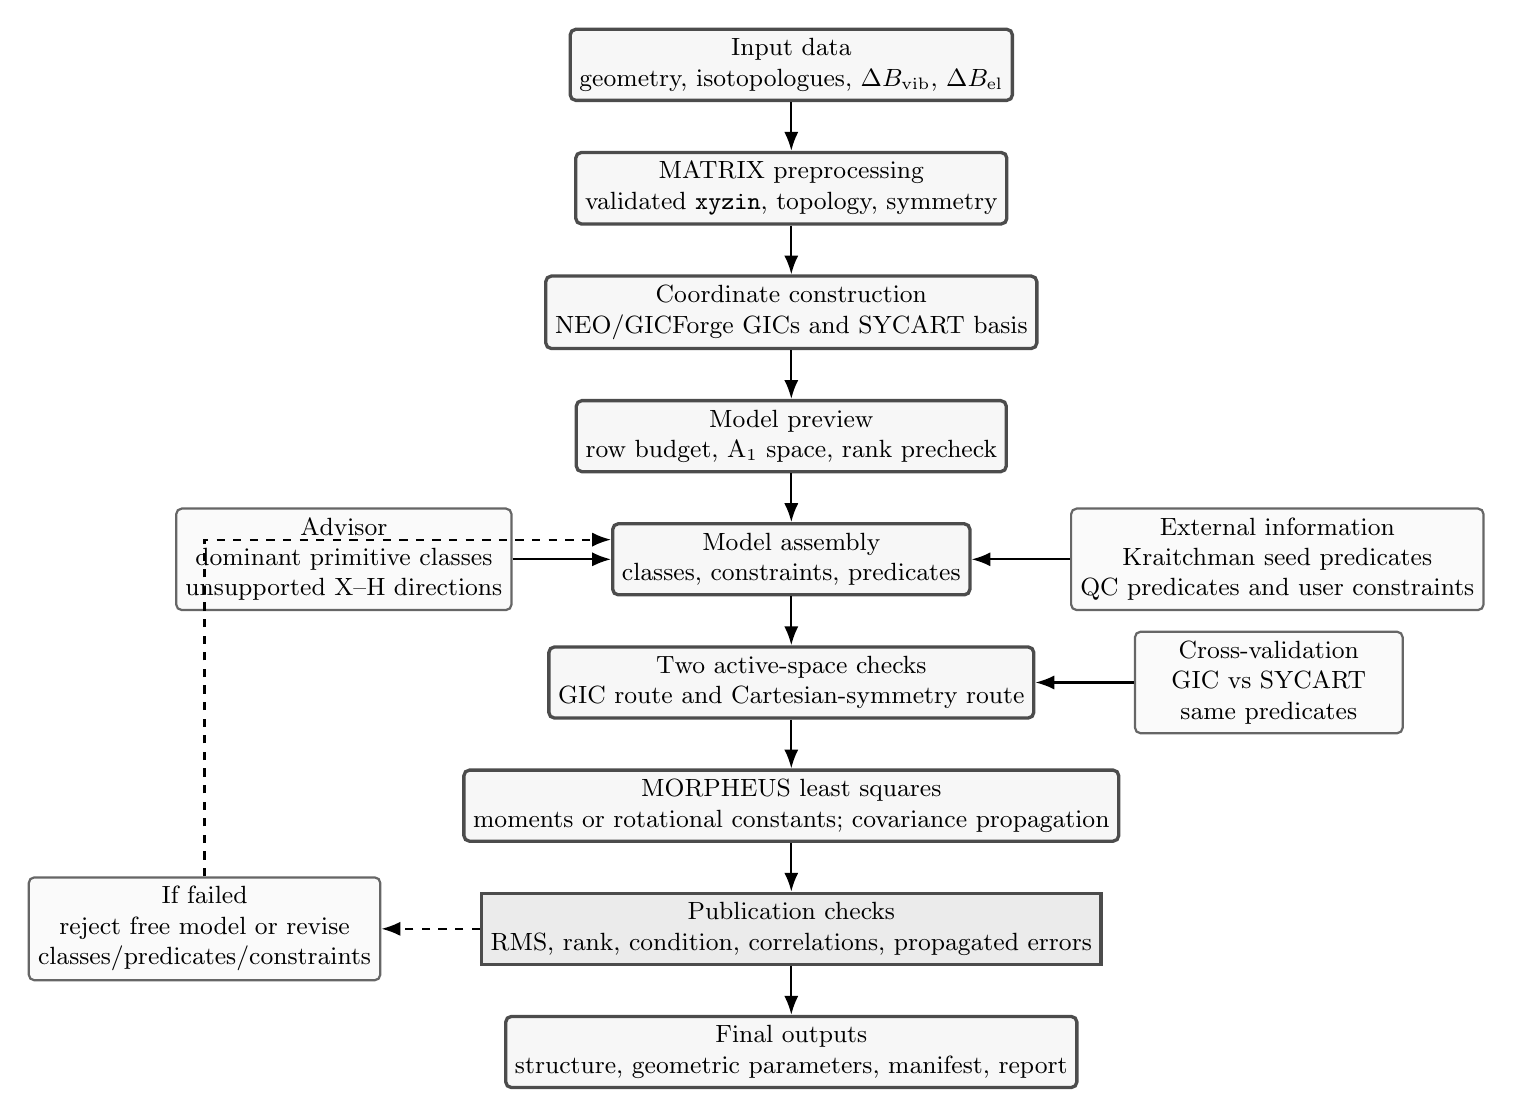
\begin{tikzpicture}[
  font=\small,
  node distance=0.62cm,
  box/.style={rectangle, rounded corners=2pt, draw=black!70, very thick, align=center,
              minimum width=4.2cm, minimum height=0.78cm, fill=black!3},
  side/.style={rectangle, rounded corners=2pt, draw=black!60, thick, align=center,
               minimum width=3.4cm, minimum height=0.70cm, fill=black!2},
  check/.style={rectangle, draw=black!70, very thick, align=center,
                minimum width=4.2cm, minimum height=0.78cm, fill=black!8},
  arrow/.style={-{Latex[length=2.4mm]}, thick},
  soft/.style={-{Latex[length=2.4mm]}, thick, dashed}
]
\node[box] (input) {Input data\\geometry, isotopologues, $\Delta B_\mathrm{vib}$, $\Delta B_\mathrm{el}$};
\node[box, below=of input] (pre) {MATRIX preprocessing\\validated \texttt{xyzin}, topology, symmetry};
\node[box, below=of pre] (coord) {Coordinate construction\\NEO/GICForge GICs and SYCART basis};
\node[box, below=of coord] (preview) {Model preview\\row budget, A$_1$ space, rank precheck};
\node[box, below=of preview] (model) {Model assembly\\classes, constraints, predicates};
\node[box, below=of model] (basis) {Two active-space checks\\GIC route and Cartesian-symmetry route};
\node[box, below=of basis] (fit) {MORPHEUS least squares\\moments or rotational constants; covariance propagation};
\node[check, below=of fit] (checks) {Publication checks\\RMS, rank, condition, correlations, propagated errors};
\node[box, below=of checks] (out) {Final outputs\\structure, geometric parameters, manifest, report};

\node[side, left=1.25cm of model] (advisor) {Advisor\\dominant primitive classes\\unsupported X--H directions};
\node[side, right=1.25cm of model] (prior) {External information\\Kraitchman seed predicates\\QC predicates and user constraints};
\node[side, right=1.25cm of basis] (validate) {Cross-validation\\GIC vs SYCART\\same predicates};
\node[side, left=1.25cm of checks] (reject) {If failed\\reject free model or revise\\classes/predicates/constraints};

\draw[arrow] (input) -- (pre);
\draw[arrow] (pre) -- (coord);
\draw[arrow] (coord) -- (preview);
\draw[arrow] (preview) -- (model);
\draw[arrow] (model) -- (basis);
\draw[arrow] (basis) -- (fit);
\draw[arrow] (fit) -- (checks);
\draw[arrow] (checks) -- (out);
\draw[arrow] (advisor) -- (model);
\draw[arrow] (prior) -- (model);
\draw[arrow] (validate) -- (basis);
\draw[soft] (checks.west) -- (reject.east);
\draw[soft] (reject.north) |- ($(model.west)+(0,0.25)$);
\end{tikzpicture}%
}
\caption{Suggested MORPHEUS workflow for semiexperimental structure refinement.
The central vertical path is the reproducible pipeline; side boxes supply model-building
information or validation.  Kraitchman coordinates enter as experimental seed predicates,
not as exact constraints.}
\label{fig:morpheus-workflow}
\end{figure}

\section{Coordinate models}
\subsection{Symmetry-adapted GICs}
The default MORPHEUS active space is the non-redundant totally symmetric block of the
GIC set generated by NEO/GICForge.  Primitive coordinates are generated from topology,
reduced to a non-redundant set, symmetry-adapted, and labelled.  The active coordinates
include stretches, bends, torsions, out-of-plane coordinates, ring puckering coordinates,
and special coordinates when present.  The GIC route has three advantages:
\begin{itemize}
  \item chemical constraints can be projected directly from primitive coordinates;
  \item parameter classes can be defined in chemically meaningful families;
  \item propagated errors can be reported for bond lengths, angles, torsions, and ring
        puckering coordinates.
\end{itemize}

\subsection{Symmetry-adapted Cartesians}
The alternative active space is a symmetry-adapted Cartesian displacement basis after
removal of translations and rotations.  This route is useful as an independent numerical
check because it avoids possible bias from a particular internal-coordinate reduction.
It is less transparent chemically: primitive constraints and predicates can still be
projected onto the Cartesian basis, but the fitted parameters themselves are Cartesian
symmetry displacements, not local structural variables.

\subsection{Expected equivalence}
For a well-posed least-squares model, the two active spaces should give the same final
observable residuals and the same structural corrections within numerical tolerance.
Differences are meaningful diagnostics.  A large difference indicates an ill-posed
model, an incomplete constraint projection, a singular coordinate block, or a mismatch
between chemical priors and experimental information.

\section{Model choices}
\subsection{Fully free refinement}
The fully free model is the least biased option, but it is rarely meaningful unless the
number and distribution of isotopologues are sufficient.  MORPHEUS now rejects an
underdetermined free refinement before iteration.  This is essential: a formally small
rotational RMS is not a structural result if unsupported directions are present.

\subsection{Hard constraints}
Hard constraints remove directions from the active least-squares space.  They are
appropriate when a coordinate is known not to be determined by the data, for example
unsubstituted hydrogen local frames in a heavy-atom isotopic dataset.  Hard constraints
must be reported because they have zero variance along the removed directions.

\subsection{Parameter classes}
Parameter classes tie several corrections to one fitted variable.  They do not force
the final primitive values to be identical; they force their corrections from the
reference structure to share one amplitude.  Classes are useful when the data support a
family correction but not each member separately.  Examples are CC stretches, CO
stretches, chemically related valence angles, or terminal CH$_2$ stretches.
In the automatic mode these families are generated from continuous MATRIX synthons
rather than from rigid element labels alone.  The synthon thresholds control how
finely covalency, delocalization, strain, and bond order are resolved.  MORPHEUS
tests coarse, medium, and fine partitions and selects the simplest candidate that
passes rank and propagated-uncertainty checks.

\subsection{Predicates}
Predicates are weighted structural observations, not exact constraints.  They are the
preferred way to use high-quality reference structures when the rotational data alone
do not determine all directions.  A distance predicate with $\sigma=0.003$~\AA{} and
an angle predicate with $\sigma=0.3^\circ$ mean that deviations are allowed but penalized
according to the stated uncertainty.  The covariance matrix includes the predicate
weights, so final structural uncertainties are propagated rather than estimated by
Monte Carlo sampling.

The distance-predicate and advisor thresholds are intentionally class dependent.  A
bond between two non-hydrogen atoms is denoted here as an XY bond.  An X--H bond is
not treated as a single universal class: C--H bonds are separated from all other X--H
bonds.  Non-CH X--H bonds are scored with the same propagated-uncertainty threshold
as XY bonds, because they may be directly constrained by isotopic substitution,
Kraitchman information, or reliable local chemistry.  C--H distances, in contrast,
often lack deuterated isotopologues in practical datasets and are weakly determined
by heavy-atom substitutions.  MORPHEUS therefore uses a broader acceptance threshold
for C--H distances in the automatic model selector.  This distinction prevents the
selector from rejecting an otherwise well-conditioned chemically meaningful model
only because unsupported C--H directions have larger propagated errors, while still
requiring non-CH X--H and XY distances to meet the tighter structural criterion.

\subsection{Kraitchman-derived predicates}
Single-substitution Kraitchman coordinates provide an independent experimental
geometric seed.  MORPHEUS writes both a Kraitchman comparison table and, when possible,
a principal-axis seed geometry.  This seed can now be converted into local primitive
predicates.  The conservative default generates a predicate only when every atom in
the primitive coordinate has a Kraitchman target; an optional partial mode also allows
mixed primitives containing Kraitchman-seeded atoms and reference-geometry atoms.  The
resulting predicates are labelled as \texttt{kraitchman\_seed\_distance} or
\texttt{kraitchman\_seed\_angle}.  They should normally be assigned broader uncertainties
than high-level QC predicates, because Kraitchman coordinates contain sign choices,
small-coordinate instabilities, substitution assumptions, and vibration/electronic
correction dependencies.

\subsection{Automatic advisor}
The advisor now builds disjoint suggestions from dominant primitive contributions to
each GIC.  A GIC is assigned to a synthon-derived class only when one primitive family
is dominant; classes are never allowed to mix stretches, bends, torsions, or other
coordinate types.  The refinement can be set to coarse, medium, fine, or automatic;
the automatic choice is made from candidate fits using propagated uncertainties for
XY bonds, non-CH X--H bonds, C--H bonds, and heavy-atom angles.  The default
acceptance thresholds are deliberately not identical: XY and non-CH X--H distances
share the tighter criterion, C--H distances have a wider criterion, and heavy-atom
valence angles are checked separately.  When hydrogen
substitutions are absent, dominant X--H angle directions may be proposed as fixed
directions.  The advisor is deliberately a model builder, not a black-box guarantee:
its output is validated by rank, condition number, residuals, propagated
uncertainties, and warning diagnostics.

\section{Current numerical checks}
The following tests use the fructose and deoxy-D-ribose datasets already converted to
MATRIX \texttt{xyzin}.  All fits use moments of inertia and the ABC components.

Advisor-only and X--H-blocked tests are useful diagnostics but are not reported as
structural results here.  They can give small rotational residuals while leaving
geometric uncertainties too large, especially for valence angles and torsions.  MORPHEUS
therefore treats rank, condition number, covariance propagation, and high-correlation
diagnostics as model checks rather than as replacements for chemically meaningful
geometric uncertainties.  The publishable models below use weighted structural
predicates and pass the propagated-error checks.

\begin{table}[h]
\centering
\caption{GIC versus Cartesian symmetry coordinates with the same predicate model
($\sigma_R=0.003$~\AA, $\sigma_A=0.3^\circ$, $\sigma_D=0.5^\circ$).}
\resizebox{\textwidth}{!}{%
\begin{tabular}{llrrrrrr}
\toprule
System & Coordinate model & Parameters & Rank & RMS/MHz & Condition & max $\sigma_R$/\AA & max $\sigma_A$/deg \\
\midrule
Fructose & GIC & 30 & 30 & 0.016560945 & 94.1 & 0.000301 & 0.030 \\
Fructose & Cartesian symmetry & 30 & 30 & 0.016560945 & 78.0 & -- & -- \\
Deoxy-D-ribose & GIC & 21 & 21 & 0.011124743 & 60.4 & 0.000559 & 0.055 \\
Deoxy-D-ribose & Cartesian symmetry & 21 & 21 & 0.011124743 & 54.0 & -- & -- \\
\bottomrule
\end{tabular}
}
\end{table}

With predicates the two active spaces become numerically equivalent.  The small
conditioning advantage of Cartesian symmetry coordinates in these two tests does not
remove the need for GICs, because the chemical model, the constraints, and the final
published parameters are naturally internal-coordinate quantities.

\section{Recommended workflow}
\begin{enumerate}
  \item Build topology, symmetry, and non-redundant GICs once from the validated
        \texttt{xyzin}.
  \item Preview the model: count rows, active coordinates, suggested classes, and fixed
        hydrogen directions.
  \item Reject fully free models when the row budget or rank is insufficient.
  \item Generate Kraitchman diagnostics and test Kraitchman predicates when isotope
        coverage is suitable.
  \item Try advisor-generated classes and inspect rank, condition number, propagated
        errors, and high-correlation diagnostics.
  \item Add hard constraints only for directions that are physically unsupported by the
        data.
  \item Add predicates for chemically meaningful reference information, with documented
        uncertainties.
  \item Run both GIC and Cartesian symmetry active spaces for final validation when the
        system is important enough for publication.
\end{enumerate}

\section{Final geometric parameters}
Figure~\ref{fig:morpheus-workflow} and the diagnostics above define the workflow, but
the structural result is the set of fitted geometric parameters and their propagated
uncertainties.  The following tables report the final GIC-based predicate refinements.
C--H coordinates are omitted because they are not determined by the present isotopic
datasets; O--H coordinates are retained and marked by their zero model variance when
fixed by the hydrogen-frame constraint.  Ring conformations are reported through
Cremer--Pople-like \(Q\) and \(\phi\) coordinates rather than by listing all
intracyclic torsions.

\subsection{Fructose: final geometric parameters}
\begin{landscape}
\scriptsize
\begin{longtable}{llll}
\toprule
Coordinate & Atoms & Unit & Final value \\
\midrule
\endhead
R(1,11) & C--O & \AA{} & 1.41844 $\pm$ 3.0e-04 \\
R(1,2) & C--C & \AA{} & 1.51892 $\pm$ 2.9e-04 \\
R(10,21) & O--H & \AA{} & 0.96268 $\pm$ 0.0000 \\
R(11,13) & O--H & \AA{} & 0.96166 $\pm$ 0.0000 \\
R(12,24) & O--H & \AA{} & 0.96616 $\pm$ 0.0000 \\
R(2,12) & C--O & \AA{} & 1.40861 $\pm$ 2.9e-04 \\
R(2,3) & C--C & \AA{} & 1.52438 $\pm$ 2.8e-04 \\
R(2,7) & C--O & \AA{} & 1.40764 $\pm$ 2.9e-04 \\
R(3,4) & C--C & \AA{} & 1.51998 $\pm$ 2.9e-04 \\
R(3,8) & C--O & \AA{} & 1.41741 $\pm$ 3.0e-04 \\
R(4,5) & C--C & \AA{} & 1.51817 $\pm$ 2.9e-04 \\
R(4,9) & C--O & \AA{} & 1.41636 $\pm$ 3.0e-04 \\
R(5,10) & C--O & \AA{} & 1.41247 $\pm$ 3.0e-04 \\
R(5,6) & C--C & \AA{} & 1.51383 $\pm$ 2.9e-04 \\
R(6,7) & C--O & \AA{} & 1.42288 $\pm$ 2.9e-04 \\
R(8,14) & O--H & \AA{} & 0.96415 $\pm$ 0.0000 \\
R(9,15) & O--H & \AA{} & 0.96227 $\pm$ 0.0000 \\
A(1,11,13) & C--O--H & deg & 106.745 $\pm$ 0.000 \\
A(1,2,12) & C--C--O & deg & 109.660 $\pm$ 0.027 \\
A(1,2,3) & C--C--C & deg & 113.219 $\pm$ 0.026 \\
A(1,2,7) & C--C--O & deg & 104.871 $\pm$ 0.028 \\
A(2,1,11) & C--C--O & deg & 109.162 $\pm$ 0.028 \\
A(2,12,24) & C--O--H & deg & 105.741 $\pm$ 0.000 \\
A(2,3,4) & C--C--C & deg & 110.336 $\pm$ 0.022 \\
A(2,3,8) & C--C--O & deg & 111.817 $\pm$ 0.030 \\
A(2,7,6) & C--O--C & deg & 114.620 $\pm$ 0.024 \\
A(3,2,12) & C--C--O & deg & 106.577 $\pm$ 0.027 \\
A(3,2,7) & C--C--O & deg & 110.551 $\pm$ 0.022 \\
A(3,4,5) & C--C--C & deg & 110.624 $\pm$ 0.023 \\
A(3,4,9) & C--C--O & deg & 110.420 $\pm$ 0.030 \\
A(3,8,14) & C--O--H & deg & 106.023 $\pm$ 0.000 \\
A(4,3,8) & C--C--O & deg & 110.001 $\pm$ 0.030 \\
A(4,5,10) & C--C--O & deg & 110.801 $\pm$ 0.027 \\
A(4,5,6) & C--C--C & deg & 109.079 $\pm$ 0.023 \\
A(4,9,15) & C--O--H & deg & 106.847 $\pm$ 0.000 \\
A(5,10,21) & C--O--H & deg & 106.245 $\pm$ 0.000 \\
A(5,4,9) & C--C--O & deg & 107.759 $\pm$ 0.030 \\
A(5,6,7) & C--C--O & deg & 112.280 $\pm$ 0.024 \\
A(6,5,10) & C--C--O & deg & 108.932 $\pm$ 0.030 \\
A(7,2,12) & O--C--O & deg & 112.075 $\pm$ 0.028 \\
QPck0001 & C--C--C--C--C--O & rad & 0.06526 $\pm$ 0.0008 \\
PhiP0001 & C--C--C--C--C--O & deg & -94.707 $\pm$ 0.690 \\
\bottomrule
\end{longtable}
\end{landscape}

\subsection{Deoxy-D-ribose: final geometric parameters}
\begin{landscape}
\scriptsize
\begin{longtable}{llll}
\toprule
Coordinate & Atoms & Unit & Final value \\
\midrule
\endhead
R(1,14) & C--O & \AA{} & 1.40512 $\pm$ 5.5e-04 \\
R(1,2) & C--C & \AA{} & 1.51723 $\pm$ 5.4e-04 \\
R(1,6) & C--O & \AA{} & 1.41593 $\pm$ 5.4e-04 \\
R(14,17) & O--H & \AA{} & 0.96041 $\pm$ 0.0000 \\
R(15,18) & O--H & \AA{} & 0.96295 $\pm$ 0.0000 \\
R(16,19) & O--H & \AA{} & 0.96184 $\pm$ 0.0000 \\
R(2,3) & C--C & \AA{} & 1.52476 $\pm$ 5.2e-04 \\
R(3,15) & C--O & \AA{} & 1.41232 $\pm$ 5.6e-04 \\
R(3,4) & C--C & \AA{} & 1.52472 $\pm$ 5.2e-04 \\
R(4,16) & C--O & \AA{} & 1.42460 $\pm$ 5.4e-04 \\
R(4,5) & C--C & \AA{} & 1.51347 $\pm$ 5.5e-04 \\
R(5,6) & C--O & \AA{} & 1.42712 $\pm$ 5.4e-04 \\
A(1,14,17) & C--O--H & deg & 107.896 $\pm$ 0.000 \\
A(1,2,3) & C--C--C & deg & 111.677 $\pm$ 0.040 \\
A(1,6,5) & C--O--C & deg & 113.071 $\pm$ 0.045 \\
A(2,1,14) & C--C--O & deg & 107.723 $\pm$ 0.049 \\
A(2,1,6) & C--C--O & deg & 111.703 $\pm$ 0.044 \\
A(2,3,15) & C--C--O & deg & 111.373 $\pm$ 0.055 \\
A(2,3,4) & C--C--C & deg & 109.895 $\pm$ 0.043 \\
A(3,15,18) & C--O--H & deg & 106.121 $\pm$ 0.000 \\
A(3,4,16) & C--C--O & deg & 109.654 $\pm$ 0.048 \\
A(3,4,5) & C--C--C & deg & 109.931 $\pm$ 0.044 \\
A(4,16,19) & C--O--H & deg & 107.054 $\pm$ 0.000 \\
A(4,3,15) & C--C--O & deg & 110.117 $\pm$ 0.047 \\
A(4,5,6) & C--C--O & deg & 109.907 $\pm$ 0.043 \\
A(5,4,16) & C--C--O & deg & 110.690 $\pm$ 0.053 \\
A(6,1,14) & O--C--O & deg & 111.583 $\pm$ 0.052 \\
QPck0001 & C--C--C--C--C--O & rad & 0.18371 $\pm$ 0.0015 \\
PhiP0001 & C--C--C--C--C--O & deg & -54.055 $\pm$ 0.474 \\
\bottomrule
\end{longtable}
\end{landscape}


\end{document}
